%% ----------------------------------------------------------------
%% Thesis.tex -- MAIN FILE (the one that you compile with LaTeX)
%% ---------------------------------------------------------------- 

% Set up the document
\documentclass[a4paper, 11pt, twoside, openright]{Thesis}  % Use the "Thesis" style, based on the ECS Thesis style by Steve Gunn
\graphicspath{{res/Figures/}}  % Location of the graphics files (set up for graphics to be in PDF format)

% Include any extra LaTeX packages required
\usepackage[square, numbers, comma, sort&compress]{natbib}  % Use the "Natbib" style for the references in the Bibliography
\usepackage{verbatim}  % Needed for the "comment" environment to make LaTeX comments
\usepackage{vector}  % Allows "\bvec{}" and "\buvec{}" for "blackboard" style bold vectors in maths
\usepackage{algorithm}
\usepackage{algorithmic}
\usepackage[T1]{fontenc}

\usepackage{subcaption}
\usepackage{venturis2}
\usepackage{lmodern}
\usepackage{textcomp}    % solve issues with lmodern
\usepackage{amsfonts}
\usepackage{amsmath}
\usepackage{amsthm}
\usepackage{mathrsfs}
\usepackage{amssymb}
\usepackage{microtype}   % better typesetting with pdfLaTeX
\usepackage{ps4pdf}

\usepackage{verbatim}
\usepackage{algorithm}
\usepackage{algorithmic}
\usepackage{graphicx}
\usepackage{caption}
\usepackage{mathtools}
\usepackage{color}

\usepackage{booktabs}
\usepackage{multirow}
\usepackage{blindtext}

\usepackage{csvsimple}

\title{\LaTeX}

\date{}

\newtheorem{mydef}{Definition}
\newtheorem{myex}{Example}
\newtheorem{myprob}{Problem}
\PSforPDF{
  \usepackage{pstricks}
}
\usepackage[compact]{titlesec}
\usepackage{booktabs}
\usepackage{sectsty}     % section titles in specified font face
%\usepackage{listings}
\usepackage{listingsutf8}
\usepackage{caption}
\usepackage{xcolor}

\usepackage{enumitem}
\newcommand\litem[1]{\item{\bfseries #1}} % for labeled items (see tools used)

\allsectionsfont{\sffamily}
\numberwithin{algorithm}{chapter}
\setcounter{secnumdepth}{3}
\setcounter{tocdepth}{2}
\renewcommand{\captionlabelfont}{\sffamily\bfseries}
\newtheorem{thm}{Theorem}
\renewcommand{\algorithmicrequire}{\textbf{Input:}}
\renewcommand{\algorithmicensure}{\textbf{Output:}}
\newcommand{\term}[1]{{\sf {\small #1}}}
\hypersetup{urlcolor=black, colorlinks=false}  % Colours hyperlinks in blue, but this can be distracting if there are many links.

%global
\newcommand{\codedir}[0]{res/code}
\newcommand{\exampledir}[0]{codeexample}

% Chapter1:
\newcommand{\somecfile}{\codedir/\exampledir/rsa_crpt.c}

\newcommand{\interestingstart}{82}
\newcommand{\interestingend}{108}



\listfiles

%\usepackage[draft]{hyperref}
%\usepackage[hyperfootnotes=false,plainpages=false]{hyperref}
%% ----------------------------------------------------------------
\begin{document}
\frontmatter	  % Begin Roman style (i, ii, iii, iv...) page numbering

% Set up the Title Page
\title  {Implementing Private Set Intersection}
\authors  {Robin Gärtner}
\addresses  {\groupname\\\deptname\\\univname}  % Do not change this here, instead these must be set in the "Thesis.cls" file, please look through it instead
\UNIVERSITY {\texorpdfstring{\href{https://www.uni-saarland.de}
            {Universit\"at des Saarlandes}}
            {Universit\"at des Saarlandes}}
\faculty{MI Fakult\"at f\"ur Mathematik und Informatik}
\department{\texorpdfstring{\href{https://saarland-informatics-campus.de/}
            {Department of Computer Science}}
            {Department of Computer Science}}
\reviewers{Prof. Dr. Nico Döttling}{Prof. Dr. Nils Ole Tippenhauer}
\date       {\today}
\subject    {}
\keywords   {}
\thesistype {Bachelorthesis}
\handin     {August 18, 2021}
\ifdefined\texhash
    \version {\texhash}
\else
    \version{}
\fi
\maketitle
%% ----------------------------------------------------------------

\setstretch{1.3}  % It is better to have smaller font and larger line spacing than the other way round

% Define the page headers using the FancyHdr package and set up for one-sided printing
\fancyhead{}  % Clears all page headers and footers
\rhead{\thepage}  % Sets the right side header to show the page number
\lhead{}  % Clears the left side page header

\pagestyle{fancy}  % Finally, use the "fancy" page style to implement the FancyHdr headers
\fancyhead[RE,LO]{\sffamily\bfseries\nouppercase{\rightmark}}
\fancyhead[LE,RO]{\thepage}
%% ----------------------------------------------------------------
% Declaration Page required for the Thesis, your institution may give you a different text to place here
\vspace*{1cm}
\textbf{\large Eidesstattliche Erkl\"arung}\\[1em]
Ich erkl\"are hiermit an Eides statt, dass ich die vorliegende Arbeit selbst\"andig verfasst 
und keine anderen als die angegebenen Quellen und Hilfsmittel verwendet habe. 
\\[0.3cm]

\textbf{\large Statement in Lieu of an Oath}\\[1em]
I hereby confirm that I have written this thesis on my own and that I have not used any other media or materials than the ones referred to in this thesis.

Saarbr\"ucken, \handindate,\\[1.5cm]
\hspace*{1cm}(\authornames)\\[2cm]

\textbf{\large Einverst\"andniserkl\"arung}\\[1em]
Ich bin damit einverstanden, dass meine (bestandene) Arbeit in beiden Versionen in die Bibliothek der Informatik aufgenommen und damit ver\"offentlicht wird.
\\[0.3cm]

\textbf{\large Declaration of Consent}\\[1em]
I agree to make both versions of my thesis (with a passing grade) accessible to the public by having them added to the library of the Computer Science Department.

Saarbr\"ucken, \handindate,\\[1.5cm]
\hspace*{1cm}(\authornames)
\cleardoublepage

% END OF frontmatter.tex

%% ----------------------------------------------------------------
% The "Dedication Page"
\pagestyle{empty}  % No headers or footers for the following pages

\null\vfill\vfill\vfill\vfill\vfill
% Now comes the "Dedication Page", written in italics

Yes, you can

\vfill\vfill\vfill\vfill\vfill\vfill\null
\cleardoublepage  % Dedication page ended, start a new page


%% ----------------------------------------------------------------
\pagestyle{empty}

\mbox{}
%\clearpage
\setstretch{1.3}  % Reset the line-spacing to 1.3 for body text (if it has changed)

% The Abstract Page
\addtotoc{Abstract}  % Add the "Abstract" page entry to the Contents
\abstract{

Diese Arbeit ist eine Analyse, des in \cite{Doettling2021} vorgestellten Protokolls.
In dem Paper wurde ein verbessertes Protokoll vorgestellt, das es beliebig vielen Parteien ermöglicht, die Schnittmenge ihrer Eingabemengen sicher zu berechnen. Ein großer Teil dieser Berechnung ist die Ermittlung der Größe der Schnittmenge. Die effiziente Lösung dieses Problems ist der Fokus des Papers.\\
Um das Protokoll zu analysieren, habe ich die relevanten Teil-Protokolle wie im Paper beschrieben in Java implementiert, und die Funktionalitäten der weniger interessanten, auch schon in anderen Papern beschriebenen, Protokolle abgebildet. Zusätzlich habe ich für die grundlegenden Funktionalitäten auch eine additiv homomorphe Verschlüsselung in Java implementiert und diese so erweitert, dass sie auch Multiplikation ermöglicht.\\
Die Analyse zeigt, dass das vorgestellte Protokoll wie beschrieben funktioniert und auch effizient ist.\\
Dadurch, dass nun gezeigt ist, dass das Protokoll nützlich ist, kann nun Forschung im Bereich der secure computation weiter auf dem Protokoll aufbauen, mit der Gewissheit, dass es keine grundlegenden Fehler enthält. 

\addtocontents{toc}{\vspace{1em}}  % Add a gap in the Contents, for aesthetics

\clearpage  % Abstract ended, start a new page

%% ----------------------------------------------------------------
\pagestyle{empty}
%\mbox{}
\clearpage
\setstretch{1.3}  % Reset the line-spacing to 1.3 for body text (if it has changed)

% The Acknowledgments page, for thanking everyone
\acknowledgements{
\addtocontents{toc}{\vspace{1em}}  % Add a gap in the Contents, for aesthetics

Thanks Obama
\Blindtext

}
\clearpage
% End of the Acknowledgments

%% ----------------------------------------------------------------

\pagestyle{fancy}  %The page style headers have been "empty" all this time, now use the "fancy" headers as defined before to bring them back



%% ----------------------------------------------------------------
\lhead{\emph{Contents}}  % Set the left side page header to "Contents"
\tableofcontents  % Write out the Table of Contents

%% ----------------------------------------------------------------
\setstretch{1.5}  % Set the line spacing to 1.5, this makes the following tables easier to read
\clearpage  % Start a new page
\lhead{\emph{Abkürzungen}}  % Set the left side page header to "Abbreviations"
\listofsymbols{ll}  % Include a list of Abbreviations (a table of two columns)
{
 \textbf{Acronym} & \textbf{W}hat (it) \textbf{S}tands \textbf{F}or \\
MPCT & \textbf{M}ulty \textbf{P}arty \textbf{C}ardinality \textbf{T}esting\\
secDT & \textbf{Sec}ure \textbf{D}egree \textbf{T}est\\
OLS & \textbf{O}blivious \textbf{L}inear \textbf{S}ystem solver\\
Weitere Abkürzungen hier eintragen
 

}

%% ----------------------------------------------------------------
%\clearpage  %Start a new page
%\lhead{\emph{Symbols}}  % Set the left side page header to "Symbols"
%\listofnomenclature{lll}  % Include a list of Symbols (a three column table)
%{
% symbol & name & unit \\
%$a$ & distance & m \\
%$P$ & power & W (Js$^{-1}$) \\
%& & \\ % Gap to separate the Roman symbols from the Greek
%$\omega$ & angular frequency & rads$^{-1}$ \\
%}
%% ----------------------------------------------------------------
% End of the pre-able, contents and lists of things
% Begin the Dedication page

\setstretch{1.3}  % Return the line spacing back to 1.3

%\pagestyle{empty}  % Page style needs to be empty for this page

\addtocontents{toc}{\vspace{2em}}  % Add a gap in the Contents, for aesthetics


%% ----------------------------------------------------------------
\mainmatter	  % Begin normal, numeric (1,2,3...) page numbering
\pagestyle{fancy}  % Return the page headers back to the "fancy" style

% Include the chapters of the thesis, as separate files
% Just uncomment the lines as you write the chapters




%%%%%%%%%%%%%%%%%%%%%%%%%%%%%%%%%%%%%%%%%%%%%%%%%%%%%%%%%%%%%%%%%%%%%%%%%%%%%%%%%%%%%%%%%%%%%%%%%%%%%%%%%%%%%%%%%%%%%%%%%%%%%%%%%

\chapter{Einführung}
Secure Multiparty Computation ist ein großes Forschungsfeld in der Kryptographie. In diesem Bereich begann die Forschung zwar schon in den 1980er Jahren, unter anderem mit Arbeiten von Yao \cite{Yao1982}, seit den 2000er Jahren bekommt die Secure Computation jedoch deutlich mehr Aufmerksamkeit. Das ist unter anderem im Anstieg der Anzahl der Veröffentlichungen pro Jahr in diesem Bereich zu sehen \cite{Kogan2021}. 
In diesem Forschungsfeld werden Methoden erforscht, mit denen gemeinsam Funktionen von Eingabedaten berechnet werden können, ohne dass dabei die anderen teilnehmenden Parteien die Eingabedaten erhalten.\\
Die Forschungen in den 80er Jahren haben die theoretischen Grundlagen der Forschung geliefert und sich beispielsweise damit beschäftigt, welche Berechnungen überhaupt möglich sind. Die Forschung in den letzten Jahren ist jedoch eher praktisch, das Ziel ist es also die Fortschritte auch in Anwendungen nutzbar zu machen \cite{Kogan2021}.\\
Durch mehrere Effekte wurden die Berechnungen erst in breiteren Anwendungsbereichen sinnvoll nutzbar. Einerseits wurden die berechnenden Computer stärker, beispielsweise hat sich unter Anderem die CPU Geschwindigkeit in PCs ungefähr verdoppelt. Das allein kann aber noch nicht die mehr als 60.000 fache Beschleunigung der Berechnungsgeschwindigkeit \cite{Kogan2021} erklären. 
\begin{figure}[H]
\begin{center}
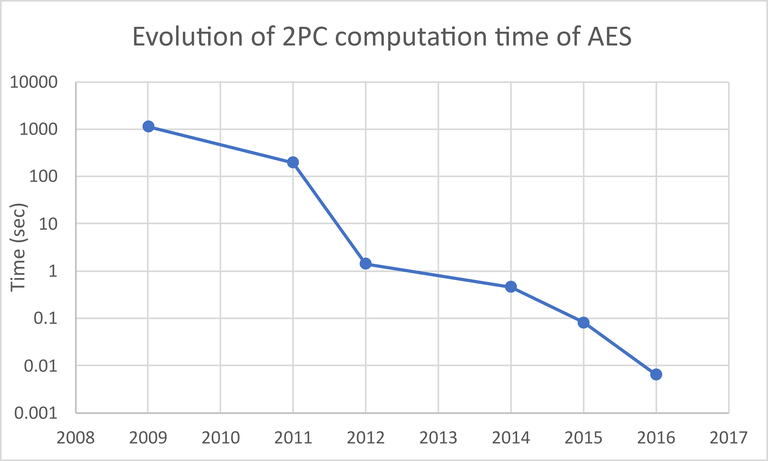
\includegraphics[width = 8cm]{comptime.png}
\caption{
Die Grafik \ref{evolution_of_computation} stellt dar\, wie sich die Geschwindigkeit der Secure Computation über die Jahre verändert hat.
Auf der Y-Achse die Berechnungszeit in Sekunden in einer logarithmischen Skala angegeben. Abgebildet ist, wie lange das zu diesem Zeitpunkt schnellste Secure Computation Protokoll für die Berechnung von AES bei der Beteiligung von zwei Parteien benötigt.\\
}
\cite{Kogan2021}
\label{evolution_of_computation}
\end{center}

\end{figure}

Durch die Grafik \ref{evolution_of_computation} wird die sich immer weiter verbessernde Geschwindigkeit der Secure Computation Protokolle deutlich. Zur leichteren Lesbarkeit und besseren Vergleichbarkeit zeigt die Grafik zwar nur die Berechnungszeiten für zwei Parteien, dennoch wird deutlich, dass sich durch die Forschung in diesem Bereich die Effizienz von Secure Computation Protokollen stark gesteigert hat. Der größte Teil des Tempogewinns liegt also an den neu entwickelten oder verbesserten Protokollen.\\
Eine Funktion, die in vielen Bereichen interessant sein kann, ist die Schnittmenge der Eingabemengen der teilnehmenden Parteien, auch PSI für \glqq Private Set Intersection\grqq{} genannt. 2021 veröffentlichten Branco et al. \cite{Doettling2021} ein Paper, in dem ein neues Protokoll vorgestellt wurde, das die threshold-Variante dieser Funktion erfüllt. Durch eine Effizienzanalyse kann man nun feststellen, wie schnell dieses Protokoll in der Praxis sein kann.

\section{Anwendungsbeispiel}
Die Entwickler des Tor Browser, den Menschen benutzen können, um in das sogenannte Darknet zu gelangen, legen einen sehr großen Wert auf die Sicherheit der Nutzer. Das macht die Analyse bestimmter Statistiken sehr schwierig. Deshalb gibt es auch vom Anbieter selbst keine genauen Angaben über beispielsweise die Nutzerzahl, sondern nur Schätzungen. Um genauere Schätzungen über die Nutzerzahl zu ermöglichen, könnte man nun Daten von mehreren \glqq Knoten\grqq{} des Tor Netzwerks kombinieren. In diesem Fall möchte man gerne herausfinden, wie viele Überschneidungen es in den Daten der \glqq Knoten\grqq{} gibt, um Mehrfachzählungen zu vermeiden. Da viele Nutzer des Tor Browsers aber einen sehr großen Wert auf Sicherheit legen, möchte man natürlich vermeiden, Daten von mehreren \glqq Knoten\grqq{} miteinander zu kombinieren, weil so möglicherweise Informationen gewonnen werden könnten, die geheim bleiben sollten.\\
Um zu garantieren, dass die Daten beispielsweise nur zur Ermittlung der Größe der Schnittmenge genutzt werden, können spezielle Protokolle genutzt werden, die die Daten nur verschlüsselt benutzen und nur ganz bestimmte  Analysen der verschlüsselten Daten erlauben. So kann man Statistiken über das Netzwerk des Tor Browsers erstellen, ohne dass die Gefahr besteht, dass Informationen der Nutzer zugänglich werden.

\section{Zielsetzung}
Das Ziel der Arbeit ist es, die praktische Effizienz und Geschwindigkeit der im Paper von Branco et al. \cite{Doettling2021} vorgestellten neuen Teilprotokolle zu testen. \\
Um alle Teilprotokolle wie im Paper beschrieben zu implementieren, sind auch Implementierungen von anderen Veröffentlichungen nötig (\cite{Schoenmakers} Beispielsweise für das secureRank Teilprotokoll). Da zu diesem Zeitpunkt noch keine derartigen Implementierungen veröffentlicht sind, kann ich auch nicht auf diese zurückgreifen. Um die Teilprotokolle, die im Paper von Branco et al. \cite{Doettling2021} beschrieben sind, trotzdem analysieren zu können, habe ich die Unterprotokolle, die auf solche externen Paper zurückgreifen auf unsichere Weise implementiert. Das heißt, dass in meiner Implementierung dieser Teilprotokolle auch der Secret Key der Verschlüsselung benutzt wird, um Informationen zu entschlüsseln. Danach kann man dann übliche Algorithmen nutzen, um das korrekte Ergebnis der Berechnung zu erhalten, das dann wieder verschlüsselt wird.\\
Diese anderen Veröffentlichungen ebenfalls selbst zu implementieren würde über den Rahmen dieser Arbeit hinaus gehen. Für die genutzten Funktionen der Paper gibt es jedoch Schätzungen, die es ermöglichen, die Berechnungsdauer vorherzusagen.\\
Durch diese Nachbildung der Funktionalität kann das Protokoll getestet werden und die Tests können zumindest genaue Daten für die Berechnungen in den korrekt implementierten Protokollen geben.
 % 

\chapter{Grundlagen}


\section{Homomorphe Verschlüsselungen}
Homomorphe Verschlüsselung ist eine Form der Verschlüsselung, die bestimmte Berechnungen auf verschlüsselten Daten erlauben, und dann ein verschlüsseltes Ergebnis zurückgibt. Wenn dieses dann wieder entschlüsselt wird, ist das Ergebnis das gleiche, wie wenn diese Arbeitsschritte auf dem unverschlüsselten Anfangswert ausgeführt worden wären. \cite{Yi2014} \\
In dieser Arbeit wird im speziellen additiv homomorphe Verschlüsselung benutzt. Diese  erlaubt das addieren von zwei verschlüsselten Zahlen und das multiplizieren einer verschlüsselten mit einer unverschlüsselten Zahl.\\
Diese Funktionalitäten sind für das Protokoll wichtig, denn in jedem Unterprotokoll wird mit verschlüsselten Daten gerechnet. Und nur so können wir trotz einer sicheren Verschlüsselung mit den Daten rechnen, ohne den Inhalt der Verschlüsselung zu kennen.
 % Background

\chapter{Multiparty Cardinality Testing}


\section{Neues am Paper}
Diese Arbeit basiert auf dem Protokoll, das in \cite{Doettling2021} vorgestellt wurde. Es gab schon vorher einige Veröffentlichungen zum Thema Private Set Intersections, auf denen das Paper aufbauen kann. Zuerst wurden Protokolle für zwei Parteien entworfen, dann auch für mehrere Parteien. Das Paper
\cite{Ghosh2019} ist die letzte Veröffentlichung, auf der das Protokoll aufbaut.\\
Die große Neuerung in der Veröffentlichung \cite{Ghosh2019} ist, dass die Kommunikations-Komplexität nun vor allem von O(t) (also dem threshold, oder der Anzahl an erlaubten Abweichungen) und nur noch logarithmisch von O(n) (also der Größe der Eingabemengen) abhängt. \cite{Ghosh2019}\\
Das von Gosh vorgeschlagene Cardinality Testing ist jedoch noch nicht  für mehrere Parteien optimiert. Daher ist das neue Protokoll zur Bestimmung der Schnittmengen-Größe die wichtigste Neuerung des Papers \cite{Doettling2021}


\section{Abwandlungen zum Paper} \label{Änderungen}
\subsection{Broadcasts}
Das Protokoll wurde offensichtlich entworfen um auch mit mehreren teilnehmenden Parteien effizient zu sein.
Das Paper \cite{Doettling2021} nutzt also in vielen Unterprotokollen Broadcast-Funktionen.

Beispiel: secRank \cite{Doettling2021}
\begin{lstlisting}[firstnumber=1]
Each party Pi broadcasts an encrypted uniformly chosen at
random unit upper and lower triangular Toeplitz matrices...
\end{lstlisting}

Beispiel: secMult \cite{Doettling2021}
\begin{lstlisting}[firstnumber=6]
Each party Pi computes [...] and broadcasts c(i).
\end{lstlisting}

Ich habe versucht, nah an die Spezifizierungen des Papers ran zu kommen, doch 
um die Implementierung des Protokolls zu vereinfachen und um das Testen der Implementierung zu erleichtern, habe ich das System etwas abgewandelt. In meiner Implementierung gibt es einen Koordinator. Dieser Koordinator erleichtert das testen enorm, denn durch ihn kann sicher gestellt werden, dass alle "verschickten" Informationen immer zum richtigen Zeitpunkt am richtigen Ziel ankommen.\\
Diese Änderung wird die Sicherheit des Protokolls nicht schwächen, weil alle Informationen, die per Broadcast verschickt werden, immer verschlüsselt sind.
Auch wenn Daten entschlüsselt werden, sind sie immer für einen Angreifer, der Informationen über die Eingabemengen erhalten will, nutzlos. Ein gutes Beispiel dafür ist das Unterprotokoll secInv \\

\begin{figure}[h]
\begin{center}
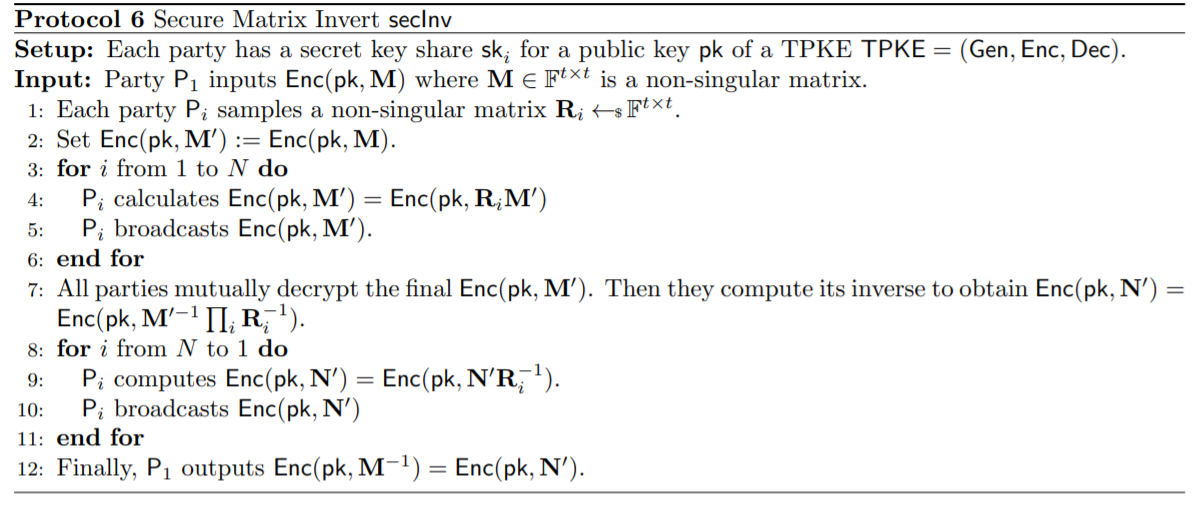
\includegraphics[width = 15cm]{secInv.png}
\caption{Teil-Protokoll secInv}
\cite{Doettling2021}
\label{oInv}
\end{center}

\end{figure}

Hier wird zwar eine Matrix entschlüsselt (7), diese ist aber randomisiert(1-5), also nutzlos, außer, man besitzt eine der geheimen Matrizen(9), die ja nicht verschickt werden.\\
Das Protokoll ist also auf eine Art und Weise aufgebaut, dass kein passiver Zuhörer irgendwelche nützlichen Informationen aus den Nachrichten, die zwischen den Parteien verschickt werden, gewinnen kann. Also kann auch ein Angreifer, der alle Nachrichten zwischen den Teilnehmern des Protokolls erhält keine Informationen extrahieren. Also können wir auch sicher sein, dass, selbst wenn der Koordinator von einem Angreifer kontrolliert wird, die verschlüsselten Eingabedaten sicher sind.\\
Die neue Struktur, die einfacher zu implementieren und testen ist, macht das Protokoll also nicht weniger sicher. Besonders deshalb, weil das Protokoll so konstruiert ist, dass selbst alle verschickten Nachrichten zusammen keine geheimen Daten preisgeben.\\

\subsection{Koordinieren der Parteien}
Die meisten der Unterprotokolle bestehen aus sich abwechselnden Teilen von Kommunikation zwischen den Parteien und Berechnungen der Parteien. Also habe ich die Unterprotokolle implementiert, indem die Berechnungen der Parteien in Abschnitte aufgeteilt sind, die dann von dem Koordinator aufgerufen werden können. Gut zu sehen ist das beispielsweise im Teil-Protokoll MPCT, wo der Koordinator nur die Koordinierung der Parteien übernimmt, indem die Parteien die richtigen Eingaben zum richtigen Zeitpunkt bekommen.\\

\begin{lstlisting}
public boolean MPCT(List<BigInteger> inputAlphas, BigInteger setMod){
        MPCTCounter++;

        List<List<EncryptedNumber>> encPointsList = new LinkedList<>();
        //line 1 already done in setup

        //line 2
        for (int i = 0; i < parties.size(); i++) {
            encPointsList.add(parties.get(i).MPCTpart1(inputAlphas, setMod));
        }
        //line 3
        return parties.get(0).MPCTpart2(encPointsList, inputAlphas, t);
    }


\end{lstlisting}

Das ist die einfachste Möglichkeit, um zu erreichen, dass alle Parteien zum richtigen Zeitpunkt das richtige Berechnen, denn einige der Berechnungen hängen auch von den gesendeten Nachrichten der anderen Parteien ab.\\


\section{andere Veröffentlichungen}
Es gibt einige andere Veröffentlichungen in den letzten Jahren, die sich mit ähnlichen Problemen oder sogar dem gleichen Problem beschäftigen.
Das Problem der Private Threshold Set Intersection lässt sich in zwei Teilprobleme aufteilen. Zum Einen in das Berechnen der Schnittmenge, worauf Gosh sich in \cite{Ghosh2019} konzentriert, und das sogar noch erweitert wurde, um auch für mehr als 2 Parteien nutzbar zu sein.\cite{Doettling2021}  Und zum anderen in der Ermittlung der Größe der Schnittmenge. Das ist der Fokus des Papers \cite{Doettling2021}. Aber auch Badrinarayanan \cite{cryptoeprint:2020:600} beschäftigt sich mit der Ermittlung der Größe der Schnittmenge. Badrinarayanan nutzt jedoch andere kryptographische Annahmen und erhält die Ergebnisse mithilfe von anderen mathematischen Grundlagen. \cite{Doettling2021}\\
Es gibt also viele neue Entwicklungen in diesem Bereich, die für unterschiedliche Zwecke genutzt, oder kombiniert werden können, um die besten Ergebnisse zu erreichen. Das Protokoll aus \cite{Doettling2021} ist also eine relevante Neuerung und eine Analyse kann helfen, die Effizienz dieser Neuerung mit anderen zu vergleichen.

 % Related Work

\chapter{Funktion der Software}

\section{Verschlüsselungen}
\subsection{Die Wahl der Verschlüsselung}
Im Paper \cite{Doettling2021} wird kein Verschlüsselungsverfahren genannt. Jedes additiv homomorphe Verschlüsselungsverfahren kann theoretisch genutzt werden. Es werden jedoch einige Vorschläge  gemacht. Einer dieser Vorschläge ist das Paillier-Kryptosystem. Das Damgard-Jurik System, für das ich mich entschieden habe, ist eine Verallgemeinerung des Paillier-Kryptosystems. Unter anderem ist die Damgard-Jurik Verschlüsselung besser für Berechnungen mit mehreren Beteiligten geeignet, denn es gibt auch eine Threshold-Variante dieses Verschlüsselungs-Systems. \cite{IvanDamgard2004}
Ich habe mich bei der Verschlüsselung für das Damgard-Jurik Cryptosystem entschieden, weil es gut zu den Anforderungen, die wir haben, passt. Es ist speziell für den Anwendungsfall mit mehreren Parteien entworfen und ist deshalb auch in unserem Fall effizient.\\



\subsection{Damgard-Jurik Verschlüsselung}
Indem wir Shamirs Secret Sharing benutzen, können wir einen public Key und eine beliebige Anzahl an Private Key-Shares erstellen. Shamirs Secret Sharing basiert auf Polynominterpolation und kann beispielsweise auch genutzt werden, um dem System später noch neue Parteien hinzuzufügen.\cite{Shamir1979}\\
Durch die Nutzung der Damgard-Jurik Verschlüsselung kann jeder, der den public Key besitzt, Daten verschlüsseln. Entschlüsseln von Daten ist jedoch komplexer. Um Daten zu entschlüsseln, müssen genügend Parteien mit Private Key-Shares die Daten teilweise entschlüsseln. Danach müssen die partiellen Entschlüsselungen kombiniert werden. Hat man aber weniger als die benötigte Anzahl an partiellen Entschlüsselungen, werden keine Informationen sichtbar. \cite{IvanDamgard2004}\\
Einer der Hauptgründe, wegen dem ich mich für die Damgard-Jurik-Verschlüsselung entschieden habe ist, das man zum Entschlüsseln von Daten den Private Key nicht wiederherstellen muss. Dadurch kann der Schlüssel nicht missbraucht werden, um auch andere Dinge zu entschlüsseln. Dadurch müssen die Parteien keiner anderen Partei trauen und die Parteien können entscheiden, was entschlüsselt werden soll und was nicht. \cite{IvanDamgard2004}\\
Die Verschlüsselung erfüllt natürlich auch die andere große Anforderung, die wir haben. Die Verschlüsselung ist additiv homomorph, was wir für die Funktionalität des Protokolls brauchen. \cite{IvanDamgard2004}

\subsection{Übertragung der Python Implementierung}
Für die Implementierung der Verschlüsselung habe ich mich an der Python Implementierung \cite{swansonk14} orientiert. Da die Sicherheit der Verschlüsselung auf mathematischen Annahmen basiert  \cite{10.1007/3-540-48910-X_16}, muss mit großen Zahlen (mehr als 32 Bits) gerechnet werden, um sicher gegen Brute-Force-Angriffe zu sein. Daher entstehen bei der Übertragung der Python Implementierung nach Java einige Probleme. Da in Python Ganzzahlen beliebig groß werden können, aber in Java Ganzzahlen auf 32 Bit begrenzt sind, muss ich auf BigInteger zurückgreifen, um verschlüsselte Zahlen korrekt darstellen zu können.
Ein ähnliches Problem ist beispielsweise das Erstellen von zufälligen Primzahlen von bestimmter Länge. In Python stellt das kein Problem dar, aber in Java ist das erstellen von beliebig langen Primzahlen komplizierter. Trotz dieser Probleme habe ich eine funktionierende Implementierung der Damgard-Jurik Verschlüsslung geschaffen, die ich dann nutzen kann, um die Implementierung der komplexeren Teil-Protokolle zu testen.


\section{Architektur}
\section{Ring Realisierung}
Da in vielen der Unterprotokollen (OLS, ODT, secMult, secRank, secInv, SUR) Berechnungen über endlichen Körpern stattfinden, um Korrektheit und Sicherheit zu gewährleisten, benötigen wir eine robuste und effiziente Möglichkeit, mit endlichen Körpern zu arbeiten.\\
Da wir unter anderem lineare Gleichungssysteme über endlichen Körpern lösen müssen, und es nur wenige Java-Bibliotheken gibt, die diese Funktionalität anbieten, ist die Open-Source Bibliothek JLinalg \cite{JLinAlg} gut für unseren Fall geeignet. Die Bibliothek bietet aber standardmäßig nur eingeschränkte Funktionalitäten für beliebige Körper an. Das Lösen von linearen Gleichungssystemen ist eines der Dinge, die aber nur in den  Rationalen Zahlen oder dem Körper \{0;1\} möglich sind. Daher war es augenscheinlich am einfachsten, die Bibliothek zu erweitern, indem ich eine neue Klasse erstellt habe, wodurch die Bibliothek jetzt auch andere Funktionalitäten über beliebig großen Körpern berechnen kann. Unter anderem kann so auch das lineare Gleichungssystem gelöst werden.\\

\begin{lstlisting}[caption = Ausschnitt aus Teil-Protokoll secDT]
        private FModular(BigInteger val)
        {
            value = val.mod(modulus);
        }

        public static FModularFactory FACTORY(BigInteger i) {
            modulus = i;
            return FACTORY;
        }
        @Override
        public FModular add(FModular val)
        {
            return new FModular(value.add(val.value).mod(modulus));
        }
        
        
        @Override
        public FModular subtract(FModular val)
        {
            return new FModular((value.subtract(val.value)).mod(modulus));
        }

        @Override
        public FModular multiply(FModular val)
        {
            return new FModular(value.multiply(val.value).mod(modulus));
        }
        
        @Override
        public FModular divide(FModular val)
        {
            return new FModular(value.multiply(val.value.modInverse(modulus)).mod(modulus));
        }
\end{lstlisting}


\section{sichere Matrix Berechnungen}
Das grundlegendste Teil-Protokoll, das im Paper \cite{Doettling2021} vorgestellt wird, ist das secMult Protokoll, das genutzt werden kann, um verschlüsselte Matrizen, also Matrizen mit verschlüsselten Einträgen miteinander zu multiplizieren. Das ist ein wichtiger Bestandteil des Protokolls, denn diese Funktion wird in vielen Teil-Protokollen genutzt.\\
\begin{lstlisting}[caption = Ausschnitt aus dem secRank Teil-Protokoll \cite{Doettling2021}][firstnumber=3]
        All parties mutually compute Enc(pk, N) = Enc(pk, XUML) via three invocations of FOMM.
\end{lstlisting}
Interessanterweise lassen sich dadurch auch verschlüsselte Zahlen multiplizieren, indem Matrizen mit nur einem Eintrag erstellt werden und diese dann multipliziert werden. Dadurch, dass wir nun verschlüsselte Zahlen addieren können (durch die additiv homomorphe Verschlüsselung) und wir jetzt auch verschlüsselte Zahlen multiplizieren können, erreichen wir ähnliche Funktionalität, wie bei voll-homomorpher Verschlüsselung. Um Zahlen zu multiplizieren, brauchen wir zwar die Mithilfe der anderen Parteien, aber nicht das Vertrauen der anderen Parteien. Denn die anderen Parteien müssen zwar ihren Teil des Secret-Keys benutzen, um ihren Teil zur Matrix Multiplikation beizutragen, aber durch das gewählte Verschlüsselungsverfahren müssen sie weder ihren Secret-Key-Share verschicken, noch werden Informationen über ihren Secret-Key-Share bekannt.\\
Durch die nun praktisch voll-homomorphe Verschlüsselung bekommen wir viele mathematische Möglichkeiten, die wir in den anderen Teil-Protokollen nutzen können.
Ein Beispiel für die entstandenen Möglichkeiten ist die Polynommultiplikation im Teil-Protokoll secDT \cite{Doettling2021}.

\begin{figure}[h]
\begin{center}
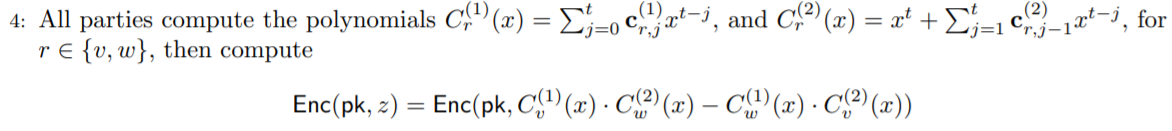
\includegraphics[width = 15cm]{secDTPart.png}
\caption{Ausschnitt aus Teil-Protokoll secDT}
\cite{Doettling2021}
\label{secDT}
\end{center}

\end{figure}

Um die verschlüsselten Polynome Cv(1) und Cw(2) miteinander zu multiplizieren, müssen wir verschlüsselte Zahlen miteinander multiplizieren. Wir können das Problem zwar teilweise umgehen, indem wir die verschlüsselten Polynome erst auswerten, wofür wir noch keine Multiplikation von verschlüsselten Zahlen nutzen müssen. In diesem Fall müssen wir aber danach die Ergebnisse der Auswertungen multiplizieren. In jedem Fall ist die Berechnung nur durch die erweiterte Funktionalität möglich.



 % Exploits

\chapter{Probleme der Software}

\section{Nicht alle Protokolle sicher implementiert}
Da einige der Protokolle auch auf anderen Veröffentlichungen basieren, für die keine Implementierungen zu finden waren, hat die Zeit nicht ausgereicht, um alle Protokolle sicher zu implementieren. Deshalb musste ich einige Teil-Protokolle unsicher implementieren, um die Funktionalität des Protokolls zeigen zu können.\\
BEISPIEL  FÜR UNSICHERE IMPLEMENTIERUNG:
OLS, braucht SUR, was auf dem Paper \cite{tcc-2007-3673} basiert.

Wenn dann die relevanten Teile der anderen Paper implementiert sind, können diese dann die unsicheren Teil-Protokolle ersetzen und diese Implementierung damit sicher machen.
Die Teil-Protokolle, bei denen eine sichere Implementierung möglich war, habe ich wie im Paper gezeigt sicher implementiert. Dazu zählen unter anderem die grundlegenden Protokolle, wie "secure Matrix Multiplikation", und die interessantesten Protokolle, wie "secure Cardinality Testing".\\



\section{Bei großen Zahlen interferieren von Ring/Verschlüsselung} % Defense

\chapter{Analyse}

\section{Die Effizienz von secDT}

\section{Die Effizienz von MPCT} % Evaluation

%\input{src/Chapters/chapter7.tex} % Discussion

\chapter{Fazit}

Das Ziel war es, zu zeigen, dass die Neuerungen aus dem Paper \cite{Doettling2021} funktionieren und effizient sind. Durch meine Implementierung der wichtigen Teilprotokolle wird deutlich, dass das im Paper \cite{Doettling2021} vorgestellte Protokoll funktioniert. \\
Die dort vorgestellten Teilprotokolle SDT und MPCT funktionieren problemlos, solange das Modulo der Verschlüsselung groß genug ist.\\
Die Analyse der Teilprotokolle MPCT und secDT hat ergeben, dass sich die Laufzeit der Protokolle wie im Paper beschrieben verhält. Die Laufzeit hängt nun also nicht mehr von der Größe der Eingabemengen ab, sondern nur von der Anzahl der "erlaubten Abweichungen" oder dem "threshold", wie er im Paper genannt wird, und der Anzahl der teilnehmenden Parteien ab. Die Anzahl der Teilnehmer hat dabei größere Auswirkungen, als der threshold.\\
Die Implementierung der additiv homomorphen Damgard-Jurik Verschlüsselung und des Teilprotokolls secMult, das auch verschlüsselte Multiplikationen ermöglicht, funktionieren ebenfalls. Dieses Teilprotokoll wird für die korrekte Funktionalität von SDT benötigt.\\
Damit kann je nach Aufgabe und Anwendungsbereich sehr viel effizienter als in früheren Protokollen festgestellt werden, ob die Schnittmenge größer ist, als ein gegebener wert. Das kann dann mit anderen Protokollen kombiniert werden, wie beispielsweise dem von Gosh und Simkin \cite{Ghosh2019} entworfenen Protokoll, um noch komplexere Protokolle effizienter zu machen. \\
Leider konnte ich durch die Zeitbegrenzung dieser Arbeit keine komplette, sichere Implementierung des ganzen vorgestellten Protokolls liefern, da zu viele der Teil-Protokolle auf die Implementierungen anderer Paper zurückgreifen, die es zu diesem Zeitpunkt noch nicht gibt.
Das Protokoll ist so nicht direkt in Anwendungen nutzbar, die auf der Datensicherheit der Eingabemengen bestehen.\\
Dennoch habe ich gezeigt, dass das Protokoll funktioniert. Dadurch kann weitere Forschung auf dem Protokoll aufbauen und es erweitern oder verbessern.\\
Das Ziel dieser Arbeit ist also erreicht, auch wenn bis zu einer sicheren Implementierung des Protokolls noch einige Arbeit nötig ist. % Conclusion

%% ----------------------------------------------------------------
% Now begin the Appendices, including them as separate files

\addtocontents{toc}{\vspace{2em}} % Add a gap in the Contents, for aesthetics

%% ----------------------------------------------------------------
%\lhead{\emph{List of Figures}}  % Set the left side page header to "List if Figures"
\listoffigures  % Write out the List of Figures

%% ----------------------------------------------------------------
%\lhead{\emph{List of Tables}}  % Set the left side page header to "List of Tables"
\listoftables  % Write out the List of Tables

\appendix % Cue to tell LaTeX that the following 'chapters' are Appendices

% Appendix A
\chapter{Additional Something}

\blindtext
\Blindtext

 % tables

\addtocontents{toc}{\vspace{2em}}  % Add a gap in the Contents, for aesthetics
\backmatter

%% ----------------------------------------------------------------
\label{Bibliography}
%\nocite{*}
%\lhead{\emph{Bibliography}}  % Change the left side page header to "Bibliography"
%\  % Use the "unsrtnat" BibTeX style for formatting the Bibliography
%\bibliographystyle{unsrtdin}
\bibliographystyle{IEEEtran}
\bibliography{src/Bibliography}  % The references (bibliography) information are stored in the file named "Bibliography.bib"

\end{document}  % The End
%% ----------------------------------------------------------------
